% This is samplepaper.tex, a sample chapter demonstrating the
% LLNCS macro package for Springer Computer Science proceedings;
% Version 2.20 of 2017/10/04
%
\documentclass[runningheads]{llncs}
\usepackage{soul}
\usepackage{tikz}
\usetikzlibrary{calc}
\usepackage{graphicx}
%\usepackage[numbers,sort&compress]{natbib}
\hyphenation{pa-ra-me-tri-za-tion}

\begin{document}
%
\title{An Event-based Architecture for Cross-Breed Multi-population Bio-inspired Optimization Algorithms}
%
%\titlerunning{Abbreviated paper title}
% If the paper title is too long for the running head, you can set
% an abbreviated paper title here
%
\author{XXXXXXXXXX\inst{1}\orcidID{0000-1111-2222-3333} \and
XXXXXXXXXX\inst{1}\orcidID{1111-2222-3333-4444} \and
XXXXXXXXXX\inst{2}\orcidID{2222--3333-4444-5555}}
%
\authorrunning{XXXXXXXXXX et al.}
% First names are abbreviated in the running head.
% If there are more than two authors, 'et al.' is used.
%
% \institute{National Technological Institute of Mexico
\institute{Hidden institute
\email{XXXXXXXXXX@XXXX.com}\\
%\url{http://www.springer.com/gp/computer-science/lncs}\\
\email{\{abc,lncs\}}}
%
\maketitle              % typeset the header of the contribution
%
\begin{abstract}
  Combining multiple algorithms, with different parameters, interacting with each
other at the same time, can benefit from the strengths of each. For instance, a
genetic algorithm could find a promising global solution that is not optimal
while another algorithm, more suitable for a local search, finds the global
optimum. This approach has been followed extensively in recent years, with
success. Moreover, there is a need for frameworks, architecture, and
implementation models that can allow researchers the development of new
parallel, asynchronous, heterogeneous, and parameter-free algorithms in a scalable way.
In this work, we present an event-driven architecture, designed to asynchronously distribute the
processing of population-based algorithms. 
The search algorithm uses a multi-population approach, creating multiple populations 
with different parameters of execution, allowing the implementation of multiple algorithms, in
this case Genetic Algorithms (GAs) and Particle Swarm Optimization (PSO).The
cross-breeding actually occurs, allowing these combined algorithms
outperform, with a high probability, single-algorithm
versions. The framework we have provided also has few parameters to
tune, since single-algorithm parameters are selected randomly; in
general, this will boost diversity of every algorithm by itself.


\keywords{Multi-population  
  \and Asynchronous 
  \and Sub-population 
  \and Serverless 
  \and Distributed.
  \and cross-breed multi-population}
\end{abstract}
%
%
%
\section{Introduction}

In the past few decades, nature-inspired optimization algorithms have been
applied to solve complex real-world problems \cite{yang2014nature}. Algorithms
inspired in natural processes include evolutionary algorithms (EAs)
\cite{back1996evolutionary} and swarm intelligence (SI) \cite{kennedy2006swarm},
among others. These population-based algorithms share the common characteristic
of using an initial set of random candidate solutions that are later used to
generate a new set of candidates, using a nature-inspired heuristic. Popular EAs
are Genetic Algorithms (GAs), Genetic Programming (GP), grey wolf optimization
(GWO) and Differential Evolution (DE), while examples of (SI) are particle swarm
optimization (PSO) and ant colony algorithms (ACO).


As in nature, population-based algorithms
are intrinsically parallel and asynchronous. Because of that, researchers have
been proposing some form of parallelization since the earlier works
\cite{muhlenbein1988evolution} with the objective of increasing the speed of
these algorithms. 
%% Island Model 
One of the first concepts proposed for parallelization was the island model,
which lead to an increased performance \cite{gorges1990explicit,grosso1985computer} 
by dividing a large population into communicated subpopulations.
%% Multi-population 
Since then, the concept has been applied to other population-based algorithms
and has been adapted by researchers to pursue other objectives besides the
execution speed. Currently, researchers use the term multi-population based
methods to describe those techniques using subpopulations as part of their
strategy.

Multi-population based methods divide the original population into
smaller subpopulations or islands, with every subpopulation carrying out the
algorithm independently, with synchronous or asynchronous communication with the
rest of the islands. This relative isolation helps in maintaining an overall
diversity since each subpopulation will search in a particular area, at least
between communications. The recombination mentioned above (mixing) or migration
between subpopulations is needed to avoid a premature convergence of candidate
solutions since smaller populations are known to perform better for a given
problem than bigger populations. However, it gives them the added advantage of
parallel operation. Additionally, and in some cases, multi-population algorithms
scale better than expected due to the interaction between the algorithm and the
parallelism of the operation \cite{ALBA20027}.

However, in most cases, algorithms applied to each subpopulation are
homogeneous, or at any rate, the same variant of the algorithm. As long as this
parallel operation is not synchronous, other population-based algorithms, or, as
a matter of fact, any algorithm, could be easily integrated. That is why several
works based on multi-population are heterogeneous, integrating various
optimization algorithms, and often performing better than single-population or
homogeneous optimization algorithms \cite{wu2016differential,nseef2016adaptive}.

Heterogeneous algorithms add another degree of freedom to the problem of finding
the correct parameter settings for an algorithm; because some parameters affect
the accuracy of the solution and the convergence speed of the algorithms as they
tip the balance between exploration and exploitation of the search space. On the
other hand, current studies show that by having a high number of subpopulations
interacting in parallel, the effect of the individual parameters of each
subpopulation is compensated by those selected in other subpopulations. In this
work, we will use random settings within a specific range as results have shown
this is a valid solution to this problem. 

Some parameters, specially the population size, are
kept fixed in order to control more easily the execution of the algorithm. For
instance, by having the size of subpopulations fixed, it is easier to control
the number of evaluations and the communication costs, when the algorithm is in
operation.

Combining multiple algorithms, with different parameters, interacting with each
other at the same time, can benefit from the strengths of each. For instance, a
genetic algorithm could find a promising global solution that is not optimal
while another algorithm, more suitable for a local search, finds the global
optimum. This approach has been followed extensively in recent years, with
success. Moreover, there is a need for frameworks, architecture, and
implementation models that can allow researchers the development of new
parallel, asynchronous, heterogeneous, and parameter-free algorithms in a scalable way.  

In this work, we present a new version of the event-driven architecture proposed
in [Anonymous]; this is a so-called {\em serverless} architecture that
asynchronously processes isolated and heterogeneous subpopulations. Each
subpopulation is treated as an event, that is pushed asynchronously into a
message queue. Events trigger stateless functions that receive the subpopulation
and proceed to run an algorithm, using the parameters and population included in
the message. After the specified number of iterations, each stateless function
returns the evolved subpopulation by again pushing a message to another queue,
used for receiving the resulting subpopulations. Subpopulations are received
from the queue by a controller that is responsible for mixing the individuals
from different subpopulations and producing new subpopulations. These new
subpopulations are pushed again by the controller into the message queue,
creating a loop. The cycle stops when the controller receives a subpopulation
containing a candidate solution that satisfies a particular condition, or a
maximum number of messages were received. 

In this new version, we propose several improvements to the original. First, we
propose alternative methods of migration between populations to compensate for
differences in the execution time of the functions. The architecture includes
external storage for the subpopulations it receives, instead of an in-process
buffer, that was limited to a small number of sub-populations. Also, the
migration or mixing process includes the capability of doing operations at the
individual-level. 
We can see the proposal as a way of evolving and mixing a
stream of populations that can very different as if their individuals belong to
different species; the term we use to describe the solution is a cross-breed
multi-population method.

To evaluate the capability of a cross-breed multi-population solution,
we conducted several experiments using different benchmark functions, comparing the
results of single versus cross-breed multi-population algorithms. For the experiments, we choose to
compare the PSO and GA algorithms, as they are well understood, and there are
several implementations in the literature. We implemented both algorithms as
stateless functions, and more algorithms can be added in the same way.

The rest of the paper is organized as follows: the next section is devoted
to analyzing the state of the art of multi-population, multi-paradigm,
stateless evolutionary algorithms. The architecture proposed is
presented in Section \ref{sec:architecture} and put to work in Section\ref{sec:exp}.
Finally, we present our conclusions and future lines of work.

\section{State of the Art}

Multi-population based methods have been used extensively in recent years, with
some journal papers dedicated exclusively to surveying the current state of the
art \cite{ma2019multi}. Furthermore,  Li et al. \cite{li2015multi} described
some of the challenges for multi-population methods in dynamic environments,
e.g., how to dynamically adapt the number populations in response to the changes
in the environment or how to determine the search area of each population. On
the subject of heterogeneous populations, a recent survey on ensemble strategies
Wu et al. \cite{wu2019ensemble} reports current advances on implementation
techniques for multi-algorithm populations. They present several works on
competitive and collaborative multi-populations as well as parametrization
techniques. Multi-population techniques are heavily applied in dynamic optimization, from
island-based parallel EAs \cite{lissovoi2017runtime}, harmony search
\cite{turky2014multi} and ACO \cite{nseef2016adaptive}. There are also 
applications to combinatorial problems \cite{pourvaziri2014hybrid}, 
and hybrid techniques using a combination of local and global operators
\cite{bai2018integrated}.

Then there are also surveys dedicated to reporting current advances in the
parallelization of particular population-based heuristics, from parallel PSO
\cite{Lalwani2019}, using GPUs in particular \cite{tan2015survey}, ACO
\cite{pedemonte2011survey} and distributed EAs \cite{gong2015distributed}.  
The most common form of parallelization is to exploit the capabilities of
multi-core CPUs and GPUs. Algorithms can run on a single workstation using a
multi-core CPU, or a GPU with multiple processing elements or in multiple
machines by using clusters, grids, or cloud services \cite{Lalwani2019}.

In this paper, we will focus on the use of cloud-based architectures that have
been used extensively in the software industry, because of their high
performance and lower overall cost. Recently, cloud providers such as Amazon Web
Services (AWS), IBM Cloud, and Google Cloud, offers a new alternative to
programming through interfaces called Serverless Computing [References]. These
platforms consist of a simple mechanism where developers can upload the code
into the service and execute it as many times as it is required, scaling and
replicating automatically, allowing a parallel execution. This way, developers
do not worry about servers, connections, and other configurations. In
serverless, users pay only for what they use. In this case, the service provides
the simple concurrent execution of stateless functions, and that is why it is
called Function as a Service (FaaS) \cite{Hellerstein2018,Baird2016}
. When using a FaaS, the client pays for every single execution of the function.
There is also the option to install some of these platforms locally; for
instance, AWS (Amazon Web Services) lambda functions \cite{Baird2016} or Apache Open Whisk
\cite{Guerv2018}. The tendency in cloud-based architectures is to move from 
monolithic to serverless architectures, in this case we are using AWS lambda
functions, as seen in Table~\ref{table:architectures}.     

\begin{table}[htp]
  \caption{Software architecture generations.}
  \label{table:architectures}
  \centering
  \begin{tabular}{|c|c|c|c|}
  \hline
  Monolithic & Microservices & Serverless \\
  \hline
  Pay for each virtual  & Pay for each  & Pay for each \\
  machine and features  & microservice  & execution \\
  \hline
  Composed by virtual servers  & Composed by virtual containers & Composed by functions \\
  Client-Server-Database & that execute small parts of a system & inside containers \\
  \hline
  OS installation required & OS only specified & OS not required\\
  \hline
  \end{tabular}
  \end{table}

%%
% SoA  for Multipopulations in Cloud 
%%

\section{Proposed architecture}
\label{sec:architecture}

Taking into account the requirements of the majority of 
multi-population methods and the advantages of cloud-native % Ref - Mario
architectures, in this paper, we propose an architecture 
that allows the scalable processing of multi-populations. 
The approach follows the best-practices of cloud-based 
distributed processing and uses a queue as the communication 
channel between computing nodes. In our case,  
each population is pushed to a queue, to be consumed by stateless functions.
Again, using a queue, populations are returned to a controller to be mixed with others.
This architecture can accept the use of an
indeterminate number of algorithms, allowing an easy cross-breed
multi-population and continuous adaptability for different problems. 
The main components of the architecture and the flow chart are shown 
in Figure~\ref{flow}.

%To develop this architecture the applied technologies are based in JavaScript
%using the NodeJS interpreter. 
% Moving to another place - Mario Explain here

\begin{figure}[htp]
  \centering
  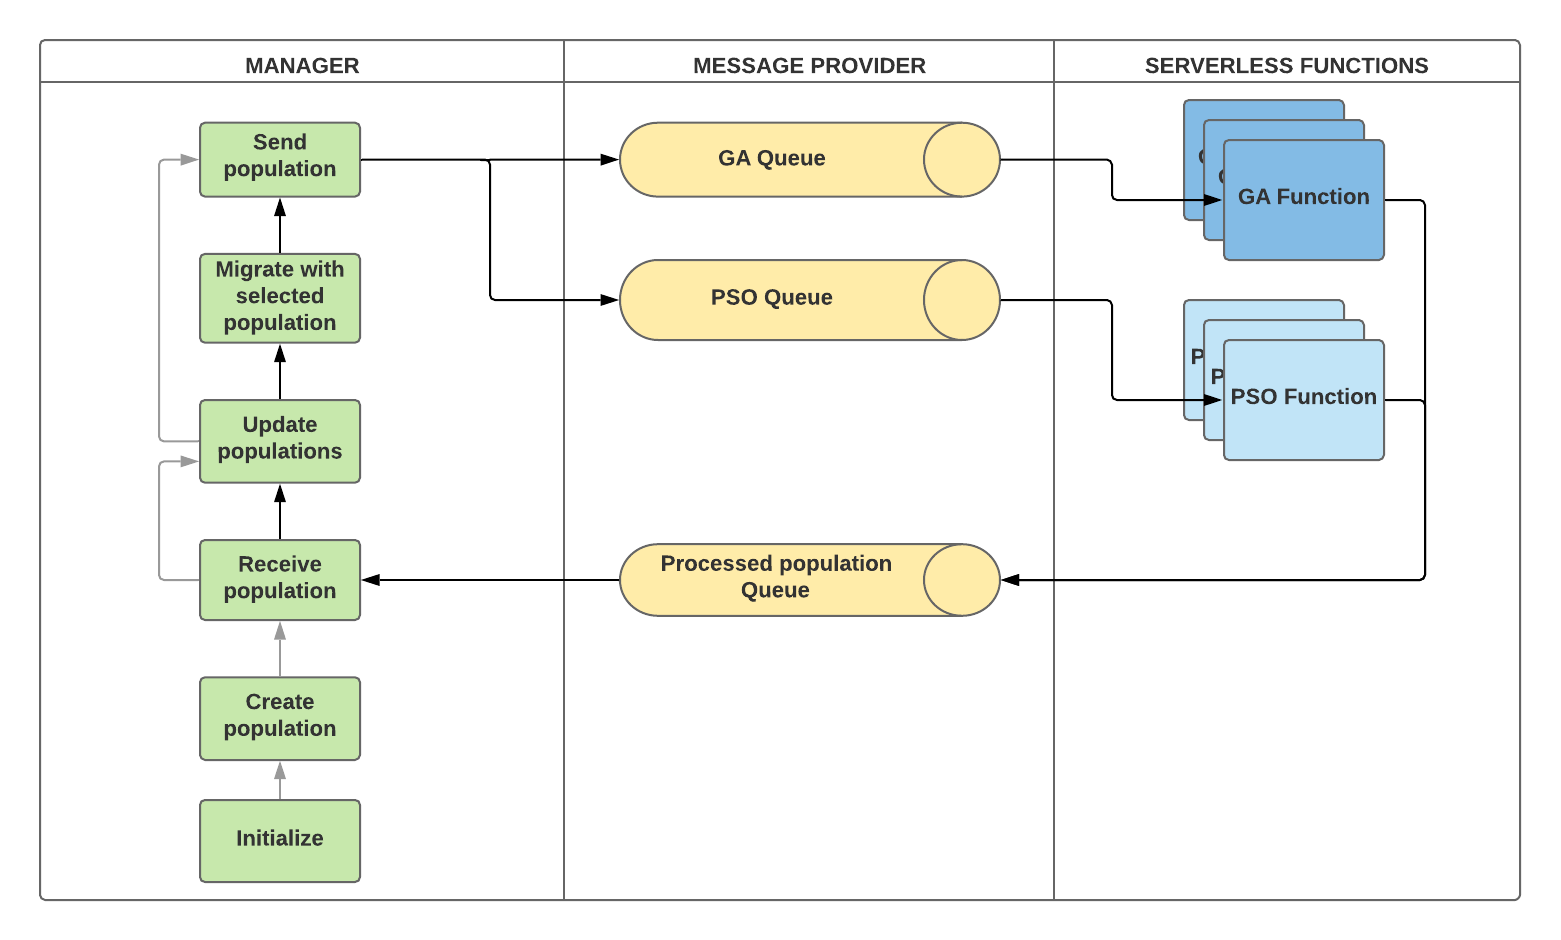
\includegraphics[width=0.9\textwidth]{img/architecture.png}
  \caption{General Architecture Flowchart.} \label{flow}
  \end{figure}

The general architecture will be described next, and then we will
focus on the most important components in the next subsections.

\subsection{Architecture}

There are three types of services in this model. First, there is a component
responsible for the management of the algorithm in general, including
starting and terminating the algorithm, and, additionally, the migration between subpopulations; this
last particular task can be decoupled in other implementations. The second service is
a message provider consisting of several scalable asynchronous queues. As a
third component, we have a collection of serverless functions. We explain the 
data flow between these services in more detail on the next subsections.  

\subsubsection{Manager}

This component receives the configuration parameters of
  the experiment and initializes it; then it proceeds to create the
  number of subpopulations needed. Every time the manager creates a new
  population, it triggers an event that stores the new population into 
  an external key-based data store implemented in MongoDB.  
  This pool of populations will be used later for in 
  the migration process. In previous works, this pool was kept in-memory and
  therefore was limited by its size. Also, the manager asynchronously 
  pushes new populations into a message queue,
  which in turn triggers a serverless function, which will be
  described below. Because each sub-population requires the execution 
  of a different algorithm in the cloud-service, there is a web socket 
  assigned for each type of algorithm, push populations to
  their respective queue.

  Once a population is processed by a stateless function, it is 
  pushed to a queue containing the processed populations. 
  The manager constantly pulls populations from this queue
  (Processed Populations queue). Each population population it takes,
  it is mixed with one of the populations stored in the population pool.
  For this, the manager takes the best two populations from
  the pool and selects one randomly. Populations in the pool are
  sorted according to their best fitness. Populations are mixed by executing
  a crossing (migration) between them; we will explain this process below. As a result of
  the migration, we have now two new populations, which are resent back
  to their respective queues. This process is repeated until the number of
  assigned migrations for the multi-population \cite{Ma2019,Santander-jim2018}
  is completed. 
  This whole
  process is performed asynchronously, avoiding the wait for all responses from
  serverless functions to perform a crossover or an update of any of the
  subpopulations \cite{Lovbjerg2001,Jimeno2019}. 

  \subsubsection{Message Provider}

  Communication is a vital aspect of distributed
systems and can be complicated to implement. Messaging systems have been used
successfully in cloud computing environments because they are scalable and
easier to use. When used as a service, they provide a secure, asynchronous, and
highly scalable mean of inter-process communication.  In this model, populations
are messages.  Messages are independent of the particular algorithm that is
going to receive them. When implemented, there are no dependencies on time,
implementation language, or operating system; systems can broadcast, publish, or
subscribe to message channels, enabling many configurations. In this
implementation,  we use only three queues, one for each type of algorithm and
one for populations returning to the manager.

\subsubsection{Serverless functions}

Population-based optimization algorithms can be implemented
as stateless functions in a serverless framework  \cite{Roberts2016},
receiving a configuration and a population as 
parameters, and returning the evolved population. 
The configuration parameter is needed because it contains all
the information needed to execute the optimization algorithm
and to report and identify the population when it is returned to the queue. 
The identifier is needed because many experiments with their corresponding 
multi-populations can be running at the same time.

% Is this why you
                                % need the "attribute" part of the
                                % population? Please say so - JJ

This operation has to be
executed in complete isolation, as a lambda function in the functional
programming paradigm, so that they are compatible with a FaaS, where serverless
functions can scale on-demand, and many copies of the same function could
working at the same time. % There needs to be a
                                % justification in terms of the
                                % algorithm for each section. Don't
                                % just say "we use this". Why is this
                                % needed? - JJ
These functions are thus ``pure'' in the functional programming term:
they have no side effects, which is why they are stateless: They
receive a sub-population, and emit another one.

This is one of the main strong points of this kind of
architecture. This lack of side effects allows easy, and automatic,
scalability, with the only bottleneck being in the message queue
itself.

\subsection{Subpopulations}

Each subpopulation is a structure with two main attributes, shown in
Figure \ref{fig4}.

\begin{itemize}
  \item {\bf Metadata}: shown as ``Attributes'' in \ref{fig4}, this
    section includes all the data needed 
  to configure and report the execution of the population.
  For instance, it has the algorithm, the parameters, objective function and 
  the optimum value (when executing benchmarks). It also includes a trace of the execution, 
  for instance, the number of evaluations per iteration, 
  the best individuals, and their fitness value.  
  It is necessary to explain that each population is independent, which means
  that even multiple benchmark functions could be optimized at the same time.
  The controller needs this data in order to migrate only populations working on
  the same problem. 
  \item {\bf Sub-population} This is the actual collection of
  individuals in the population in their current state.  
\end{itemize}
%
\begin{figure}[htp]
  \centering
  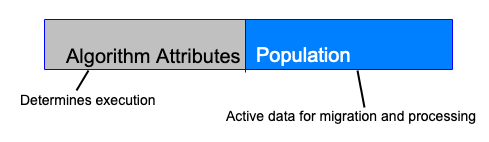
\includegraphics[width=0.5\textwidth]{img/subpopulationDefinition.png}
  \caption{Sub-population composition.} \label{fig3}
\end{figure}

% Say something about why this structure is needed and its relevance
% to the algorithm itself. Is it just administrative data, or will the
% algorithm use the attributes for something? Also why do we need this
% kind of structure. See issue #18 

\subsection{Migration} 
%
\begin{figure}[htp]
  \centering
  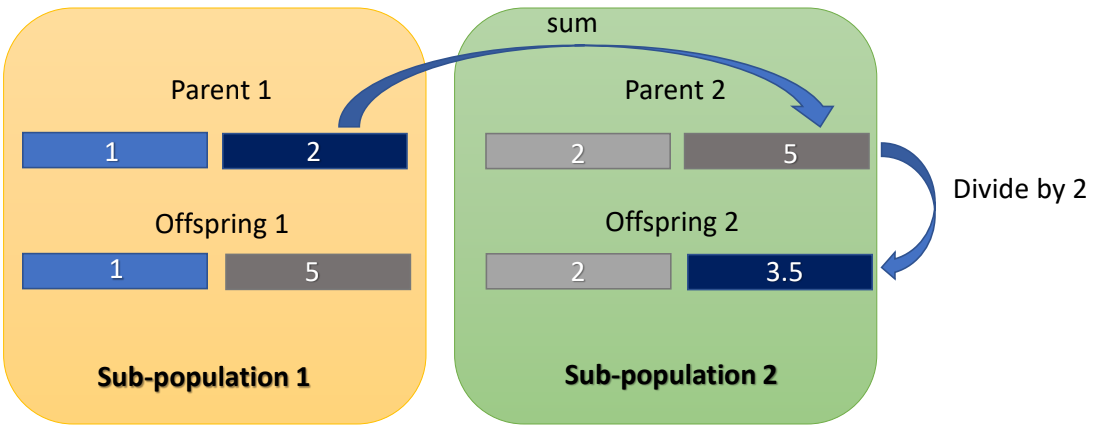
\includegraphics[width=0.9\textwidth]{img/splittinPointUniform.png}
  \caption{Splitting Point Uniform process. The offspring in
    population two gets the result of summing the corresponding gene
    of the two ancestors and dividing it by two.} \label{fig4}

\end{figure}

As we have mentioned earlier, an essential aspect of multi-population
and cross-breeding methods is the communication between subpopulations 
after several iterations of isolated
search. Individuals with some specifically chosen characteristics,
such as a high fitness, maybe combined with a certain degree of
similitude or difference to the host population, can be sent to other
population so that they keep the whole set from premature
convergence.

Our cross-breed architecture will use splitting point uniform crossover found in GA
algorithms \cite{Kramer2014}. % Found where? I have not found any reference.
This method is applied in two levels; first, when selecting which
individuals are going to migrate from one population to another, and later when
single individuals are combined. 

The method consists of applying a uniform mask created to select which elements 
are going to participate in the migration or crossover. When selected individuals are going to be
combined, the selected components, in this case, continuous values, are combined
using the midpoint between the matching genes selected by a binary mask.
\cite{Kramer2017,Kaya2011}.

We exemplified this in Figure \ref{fig4}, where we show two individuals that
were randomly selected by the uniform mask as parents of two new individuals.
Parents are shown on the top. First, the binary mask is applied. The uniform
mask assigns a 0 or 1 bit randomly to each component of the vector. Those
components having a 0 value are swapped with the other parent. For those with a
1 bit, the following operation is applied to replace the selected component in
the child: each component is combined by adding both values and then dividing
the result by two, as shown by the blue arrows. For example, for values 2 and 5,
the new value would be 3.5, as we can see in Figure \ref{fig4}. This kind of
operator is more straightforward and less explorative than BLX-$alpha$, for
instance \cite{picek2013recombination}. In our case, the exploration part is
left to the architecture itself.

\section{Experiments and Results}
  \label{sec:exp}

  In this section, we will first present the experiments that we have performed,
  including the selection of parameters, to then proceed to present and discuss
  the results in Subsection \ref{subs:results}. 
    
  \subsection{Experiments}

\begin{figure}[htp] \centering
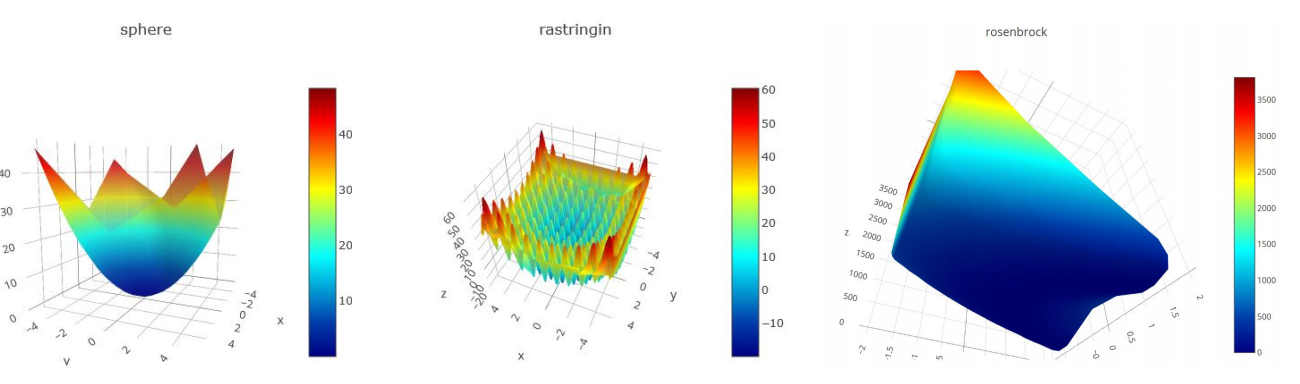
\includegraphics[width=0.7\textwidth]{img/benchmark.png} 
\caption{Benchmark
functions for experimentation.} 
\label{fig:functions} 
\end{figure}  

First, we will select those functions in which we are going to apply this framework. We
will be working on continuous optimization since they are hard optimization
problems and have also been chosen for benchmarks such as BBOB
\cite{hansen2010bbob}; out of these functions, we have chosen Rastrigin, Sphere
and Rosenbrock, which are represented in Figure \ref{fig:functions}. They have a
different degree of difficulty, can be scaled to different dimensions (as all
the rest of the benchmark functions), and they can at least give us an idea of
how single-breed (GA or PSO) algorithms perform compared to our cross-breed
(GA+PSO) version.  

   \begin{table}[h!tp]
    \caption{Parameters used by the algorithms for all dimensions.}
    \label{table:ga-pso-parameters}
    \centering
    \begin{tabular}{|l|c|c|}
    \hline
    Parameter & \multicolumn{2}{c|}{Values for dimensions} \\
      \hline
      & 2 & 10, 20, 40 \\
    \hline
    GA Generations & 50 &  70\\
    \hline
     GA Population size & 100 & 200\\
    \hline
    GA Mutation selection &  \multicolumn{2}{c|}{Tournament3}\\
    \hline
    GA Crossover selection & \multicolumn{2}{c|}{Tournament3} \\
    \hline
    GA Crossover percentage & \multicolumn{2}{c|}{Random[10\%, 80\%]} \\
    \hline
    GA Mutation percentage & \multicolumn{2}{c|}{Random[10\%,50\%]} \\
    \hline
    GA Crossover function & \multicolumn{2}{c|}{Splitting Point Uniform} \\
    \hline
    GA Mutation Function & \multicolumn{2}{c|}{Gaussian} \\
      \hline 
      \hline
    PSO Iterations & 50 & 70\\
    \hline
    PSO Vector size & 100 & 200\\
    \hline
    PSO Social factor & \multicolumn{2}{c|}{Random[0.5,4.0]} \\
    \hline
    PSO Individual factor & \multicolumn{2}{c|}{Random[0.5,4.0]} \\
    \hline
    PSO Inertia factor & \multicolumn{2}{c|}{Random[0.5,4.0]} \\
    \hline
    \end{tabular}
\end{table}

We show the parameters used for these algorithms in Table
\ref{table:ga-pso-parameters}. In every algorithm run, we will use as a stop
criteria an error below 0.5E-8. The cross-breed algorithm itself used 10
sub-populations for each experiment and a maximum of 4 migrations per
subpopulation. Since this was intended mainly as a first approach to the
performance of the cross-breed algorithm, we did not perform any optimization in
the parameter space. Note that we use random parametrization for every
population, except for the number of iterations before migration takes place and
the population size (number of initial particles in the case of PSO). 
We kept this number fixed, and also did not vary it except for the smallest case
(dimensions = 2). That was made mainly for the sake of a fair
comparison between the two algorithms. However, in principle, and as a line of
research that we could approach in the future, population size could be
random or adaptive depending on the number of dimensions.

The maximum number of evaluations follows this equation:
\begin{equation}
    \label{eq:hesitancy-interpretation}
   Evaluations = 10^{5} Dimensions
   \end{equation}
This means that evaluations will scale from 200K for the 2 dimensions,
un to 4 millions for 4 dimensions.  This kind of parametrization is
also usual in benchmarks, but of course we could use different
parameters depending on the function and scaling in a different, and
non-linear, way. 

Every experiment was carried out 15 times, using a Dell Poweredge
R730, with two Intel Xeon E5-2670v3 12-core processors, 128GB of RAM and
running Ubuntu Server 18.04 OS.

Results obtained in the experiments have been published with an open
data license in {URL hidden}

\subsection{Results}
\label{subs:results}
%
\begin{table}[h!tp]
  \caption{Experimental results. The {\bf Best} column shows in {\em
      boldface} the best value among the three algorithms, or GA-PSO
    if it is the same value as the best.}
  \label{table:resultados}
  \centering
% latex table generated in R 3.4.4 by xtable 1.8-2 package
% Thu Nov 14 13:02:26 2019
\begin{tabular}{rllrrr}
  \hline
Dimensions & Algorithm & Function & Average & SD & Best \\ 
  \hline
   2 & Rastrigin & GA & 1.65E-08 & 1.94E-08 & 0 \\ 
  2 & Rastrigin & GA-PSO & 0 & 0 & {\bf 0} \\ 
  2 & Rastrigin & PSO & 1.89E-12 & 7.31E-12 & 0 \\ 
  2 & Rosenbrock & GA & 1.24E-08 & 2.27E-08 & 1.62E-13 \\ 
  2 & Rosenbrock & GA-PSO & 6.91E-09 & 1.57E-08 & {\bf 9.58E-14} \\ 
  2 & Rosenbrock & PSO & 2.48E-06 & 9.59E-06 & 1.12E-12 \\ 
  2 & Sphere & GA & 4.37E-10 & 1.17E-09 & 4.53E-18 \\ 
  2 & Sphere & GA-PSO & 4.33E-14 & 1.37E-13 & {\bf 0 }\\ 
  2 & Sphere & PSO & 7.80E-12 & 2.06E-11 & 0 \\ 
  3 & Rastrigin & GA & 1.21E-08 & 1.98E-08 & 9.98E-13 \\ 
  3 & Rastrigin & GA-PSO & 7.72E-09 & 2.40E-08 & {\bf 0} \\ 
  3 & Rastrigin & PSO & 0 & 0 & 0 \\ 
  3 & Sphere & GA & 4.20E-11 & 1.41E-10 & 1.74E-15 \\ 
  3 & Sphere & GA-PSO & 6.28E-10 & 2.39E-09 & {\bf 0} \\ 
  3 & Sphere & PSO & 3.30E-11 & 1.18E-10 & 0 \\ 
  5 & Rastrigin & GA & 1.27E-08 & 1.48E-08 & 4.68E-12 \\ 
  5 & Rastrigin & GA-PSO & 5.57E-08 & 1.71E-07 & {\bf 0} \\ 
  5 & Rastrigin & PSO & 6.54E-01 & 1.71E+00 & 0 \\ 
  5 & Sphere & GA & 5.89E-09 & 8.62E-09 & 4.41E-11 \\ 
  5 & Sphere & GA-PSO & 8.68E-09 & 1.74E-08 & {\bf 0} \\ 
  5 & Sphere & PSO & 1.48E-03 & 5.74E-03 & 0 \\ 
10 & Rastrigin & GA & 2.38E-06 & 5.86E-06 & 3.22E-09 \\ 
  10 & Rastrigin & GA-PSO & 5.09E-09 & 1.15E-08 & {\bf 8.01E-12} \\ 
  10 & Rastrigin & PSO & 2.72E+00 & 3.87E+00 & 7.86E-11 \\ 
  10 & Rosenbrock & GA & 1.67E-04 & 2.88E-04 & 9.58E-07 \\ 
  10 & Rosenbrock & GA-PSO & 2.40E-04 & 4.63E-04 & {\bf 3.62E-07} \\ 
  10 & Rosenbrock & PSO & 4.43E+00 & 1.07E+01 & 4.17E-07 \\ 
  10 & Sphere & GA & 2.54E-08 & 2.13E-08 & 1.84E-09 \\ 
  10 & Sphere & GA-PSO & 1.30E-09 & 2.67E-09 & {\bf 3.34E-11} \\ 
  10 & Sphere & PSO & 3.08E-02 & 1.19E-01 & 4.50E-11 \\ 
  20 & Rastrigin & GA & 2.21E-01 & 4.30E-01 & 8.09E-04 \\ 
  20 & Rastrigin & GA-PSO & 7.38E-02 & 2.58E-01 & {\bf 9.13E-09} \\ 
  20 & Rastrigin & PSO & 2.55E+01 & 4.04E+01 & 3.99E+00 \\ 
  20 & Rosenbrock & GA & 1.10E-02 & 1.71E-02 & 3.48E-04 \\ 
  20 & Rosenbrock & GA-PSO & 5.61E-03 & 5.85E-03 & {\bf 2.32E-05} \\ 
  20 & Rosenbrock & PSO & 1.34E+01 & 3.68E+00 & 9.12E+00 \\ 
  20 & Sphere & GA & 9.23E-06 & 7.55E-06 & 1.85E-06 \\ 
  20 & Sphere & GA-PSO & 2.13E-08 & 2.95E-08 & 9.11E-11 \\ 
  20 & Sphere & PSO & 3.50E-07 & 9.46E-07 & {\bf 7.04E-11} \\ 
  40 & Rastrigin & GA & 3.56E+00 & 1.47E+00 & 1.95E+00 \\ 
  40 & Rastrigin & GA-PSO & 2.13E+00 & 1.83E+00 & {\bf 2.46E-04} \\ 
  40 & Rastrigin & PSO & 1.30E+02 & 1.12E+02 & 2.91E+01 \\ 
  40 & Rosenbrock & GA & 1.07E+02 & 1.66E+02 & 3.29E+01 \\ 
  40 & Rosenbrock & GA-PSO & 5.25E-01 & 4.71E-01 & {\bf 1.85E-02 }\\ 
  40 & Rosenbrock & PSO & 3.68E-01 & 3.28E-01 & 3.27E-02 \\ 
  40 & Sphere & GA & 5.30E-03 & 1.85E-03 & 2.69E-03 \\ 
  40 & Sphere & GA-PSO & 1.41E-04 & 3.63E-04 & 2.00E-10 \\ 
  40 & Sphere & PSO & 2.07E-03 & 8.01E-03 & {\bf 8.68E-11 }\\  
  \end{tabular}
\end{table}


Results are shown in Table \ref{table:resultados}, including averages
(and standard deviation) and the best results for the 15 runs. The {\bf
  Best} column show, among the 15 experiments, the best value
reached. Except for two cases, the cross-breed algorithm is either the
best or the same value as the best (in some cases where all algorithms
reach the optimum, which is 0). There are two cases where the PSO
algorithm reaches better values for the Sphere function, but in
general, we can affirm that the cross-breed algorithm proposed here
reaches either the best or a value that is very close to it.
%
\begin{figure}[h!tb]
  \centering
  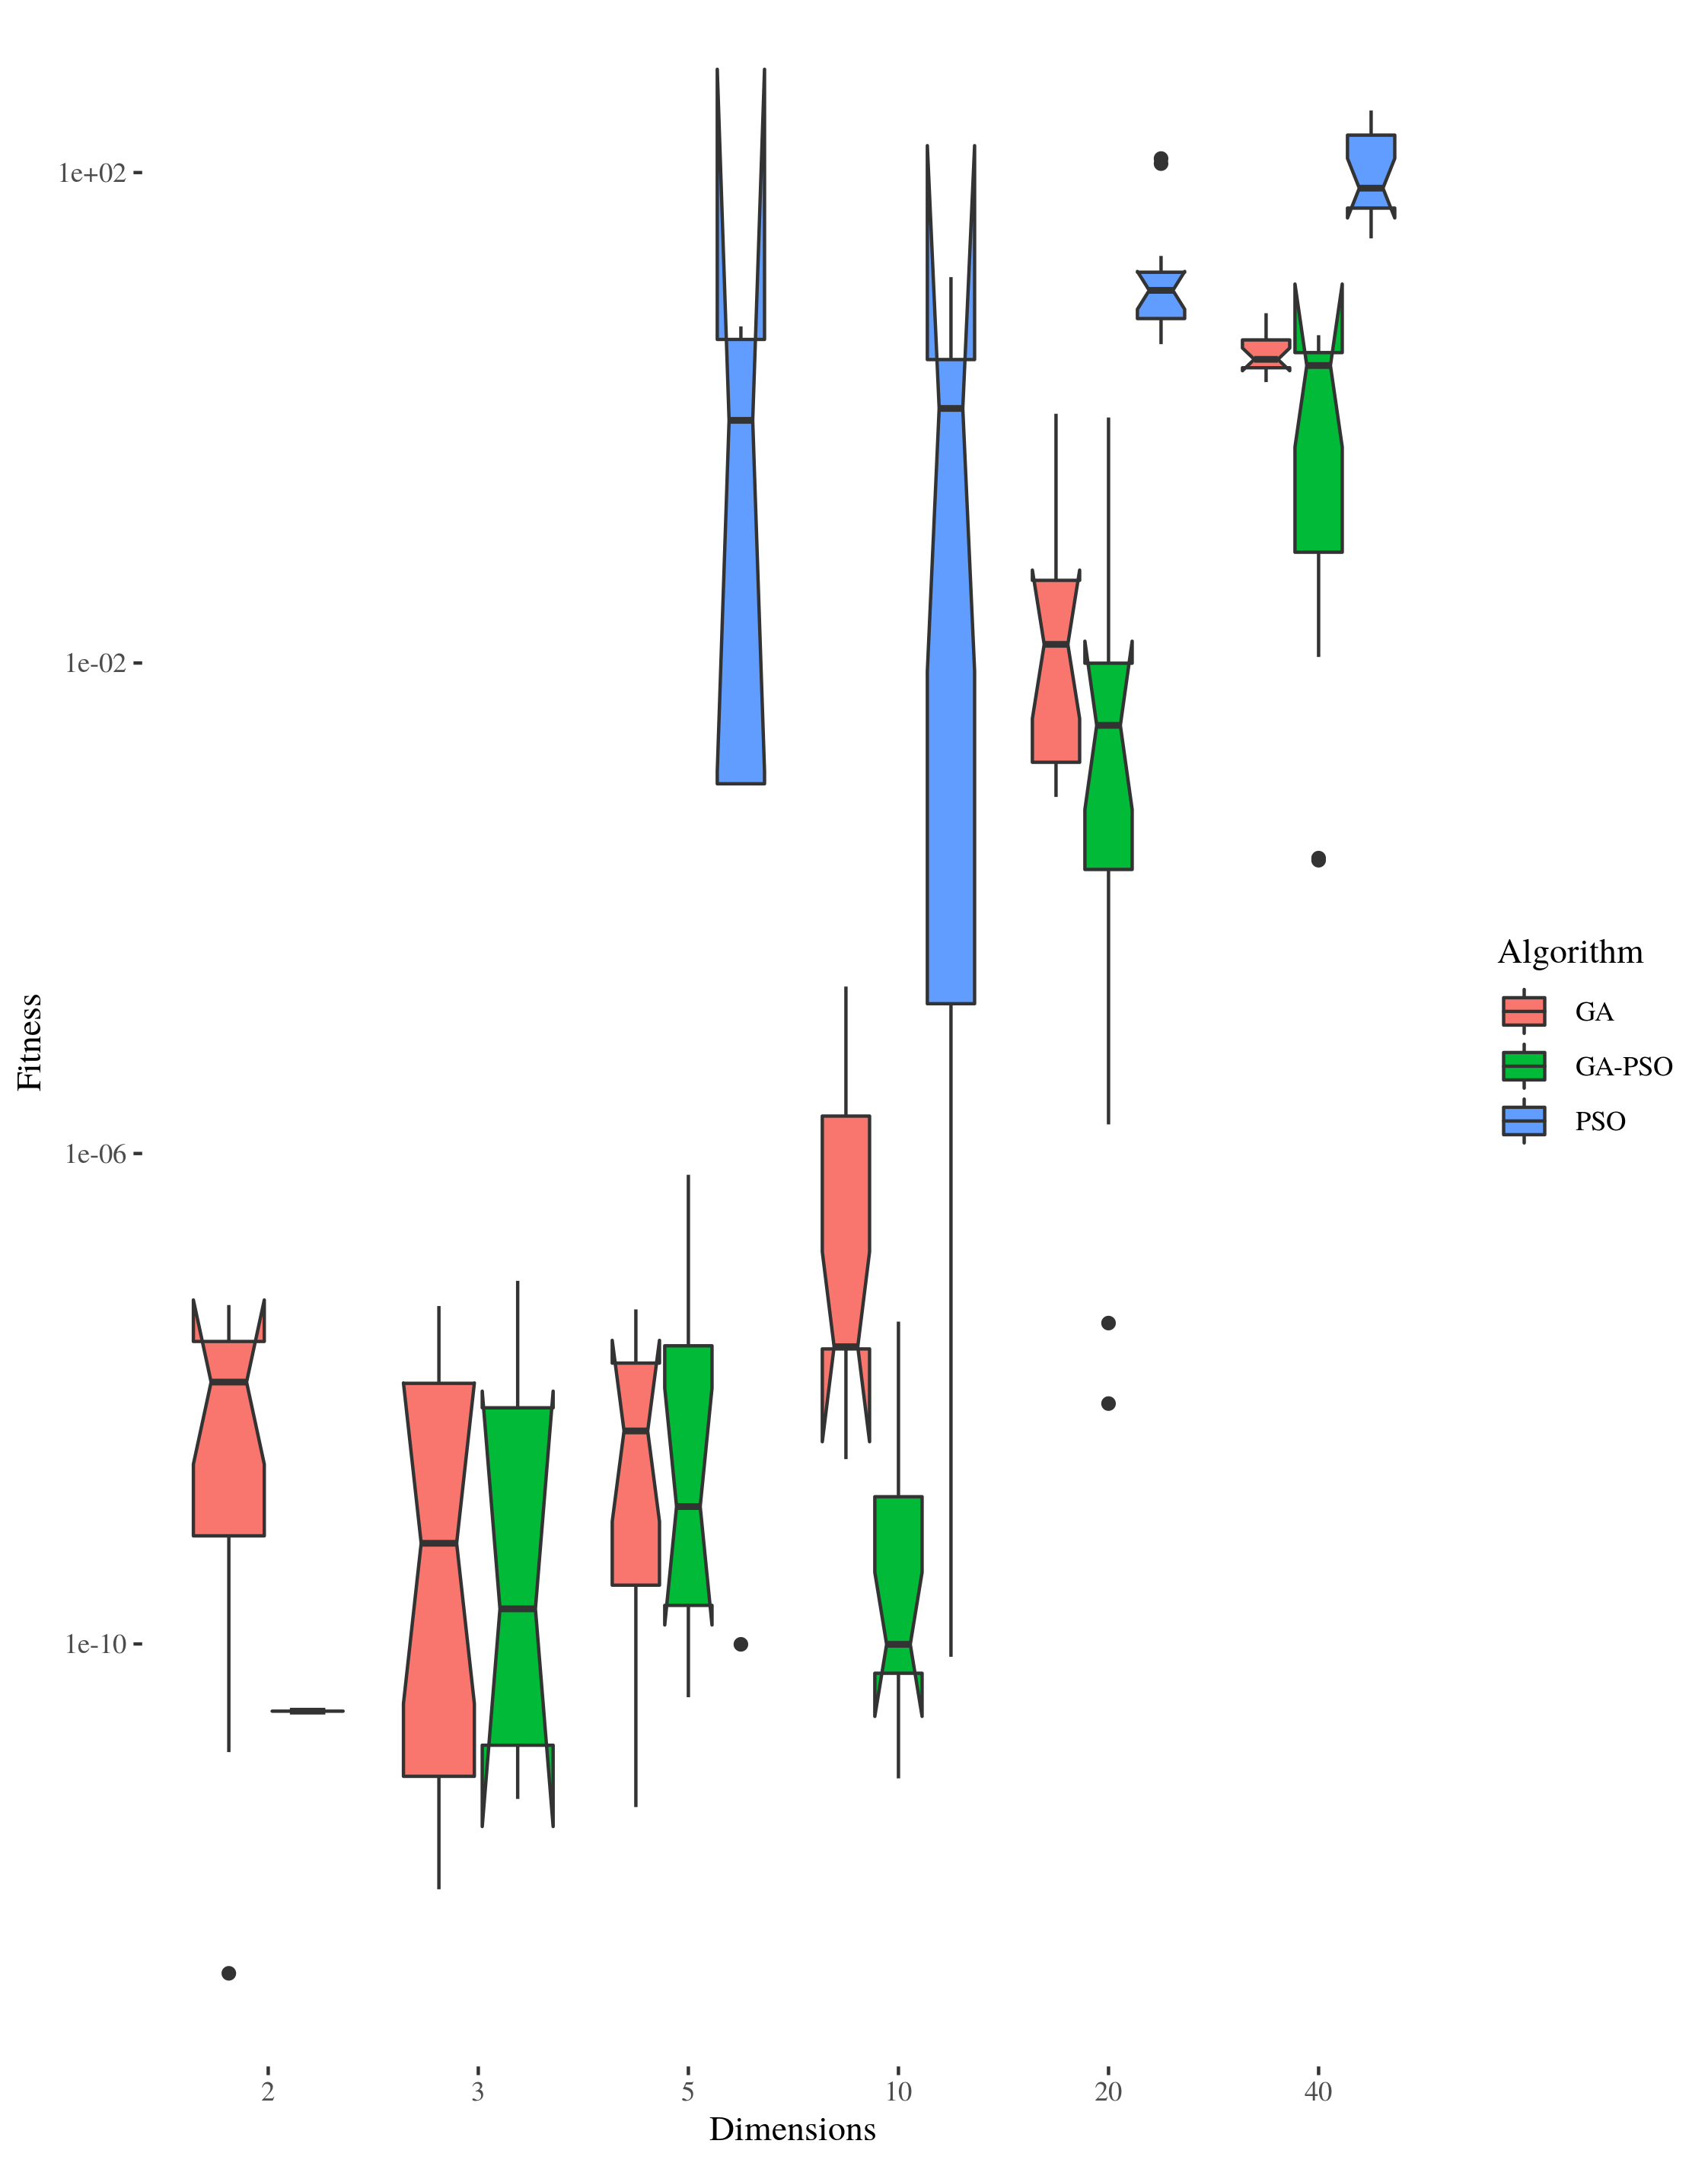
\includegraphics[height=0.4\textheight]{img/rastrigin-boxplot.png}
  \caption{Boxplots of results for the Rastrigin function. Please note the $y$ axis is logarithmic.\label{fig:boxplot:rastrigin}}
\end{figure}

Let us analyze the average behavior also via the boxplots shown
in Figure \ref{fig:boxplot:rastrigin},  \ref{fig:boxplot:sphere} and
\ref{fig:boxplot:rosenbrock}. Averages for Rastrigin are either
significantly better or similar to GAs; 10 dimensions seem to be the
case where the results for GA-PSO outperform the rest of
the algorithms significantly; they are quite similar for more dimensions and
slightly better, but similar for smaller dimensions. 

\begin{figure}[h!tb]
  \centering
  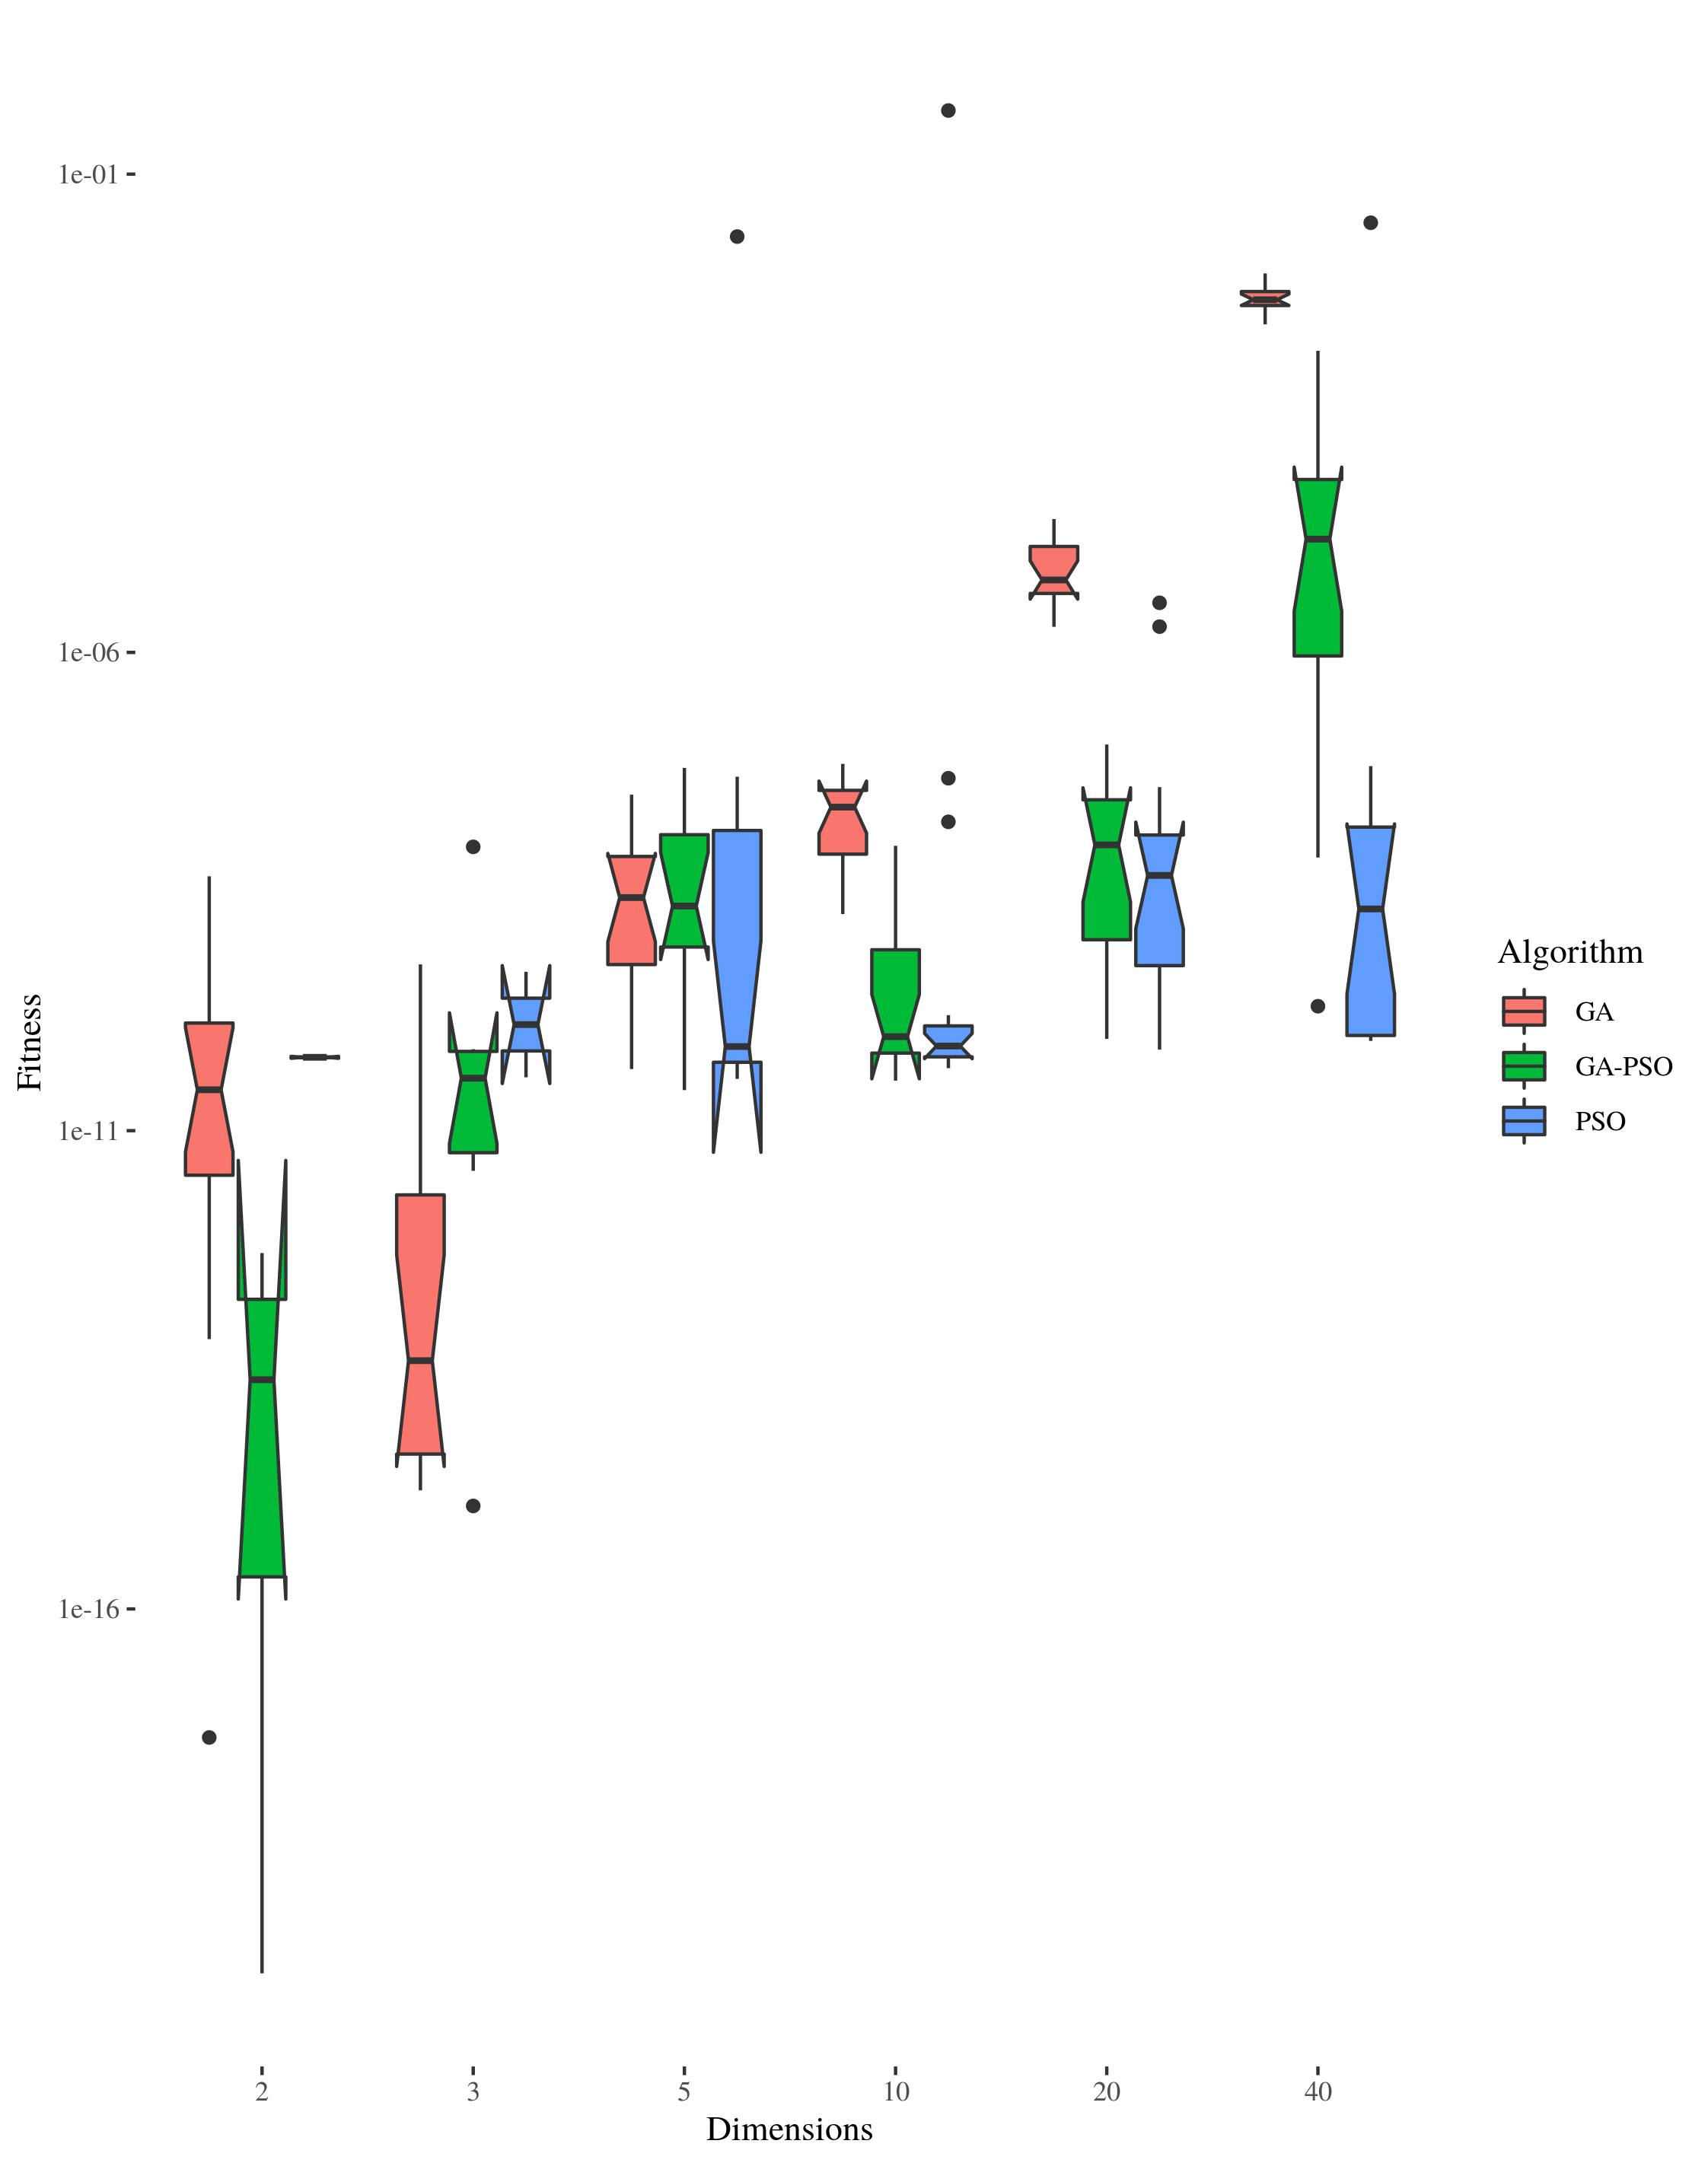
\includegraphics[height=0.44\textheight]{img/sphere-boxplot.png}
  \caption{Boxplot of results for the Sphere function, with a logarithmic $y$ axis.\label{fig:boxplot:sphere}}
\end{figure}
%
GA-PSO does not show a significant advantage for the Sphere
function, shown in Figure \ref{fig:boxplot:sphere}, except for the
smaller dimension; as the number of dimensions increases, so does the
advantage of PSO. This is probably due to the big gap between the
performance of the GA and the PSO algorithm. We will come back to this
in the discussion.
\begin{figure}[h!tbp]
  \centering
  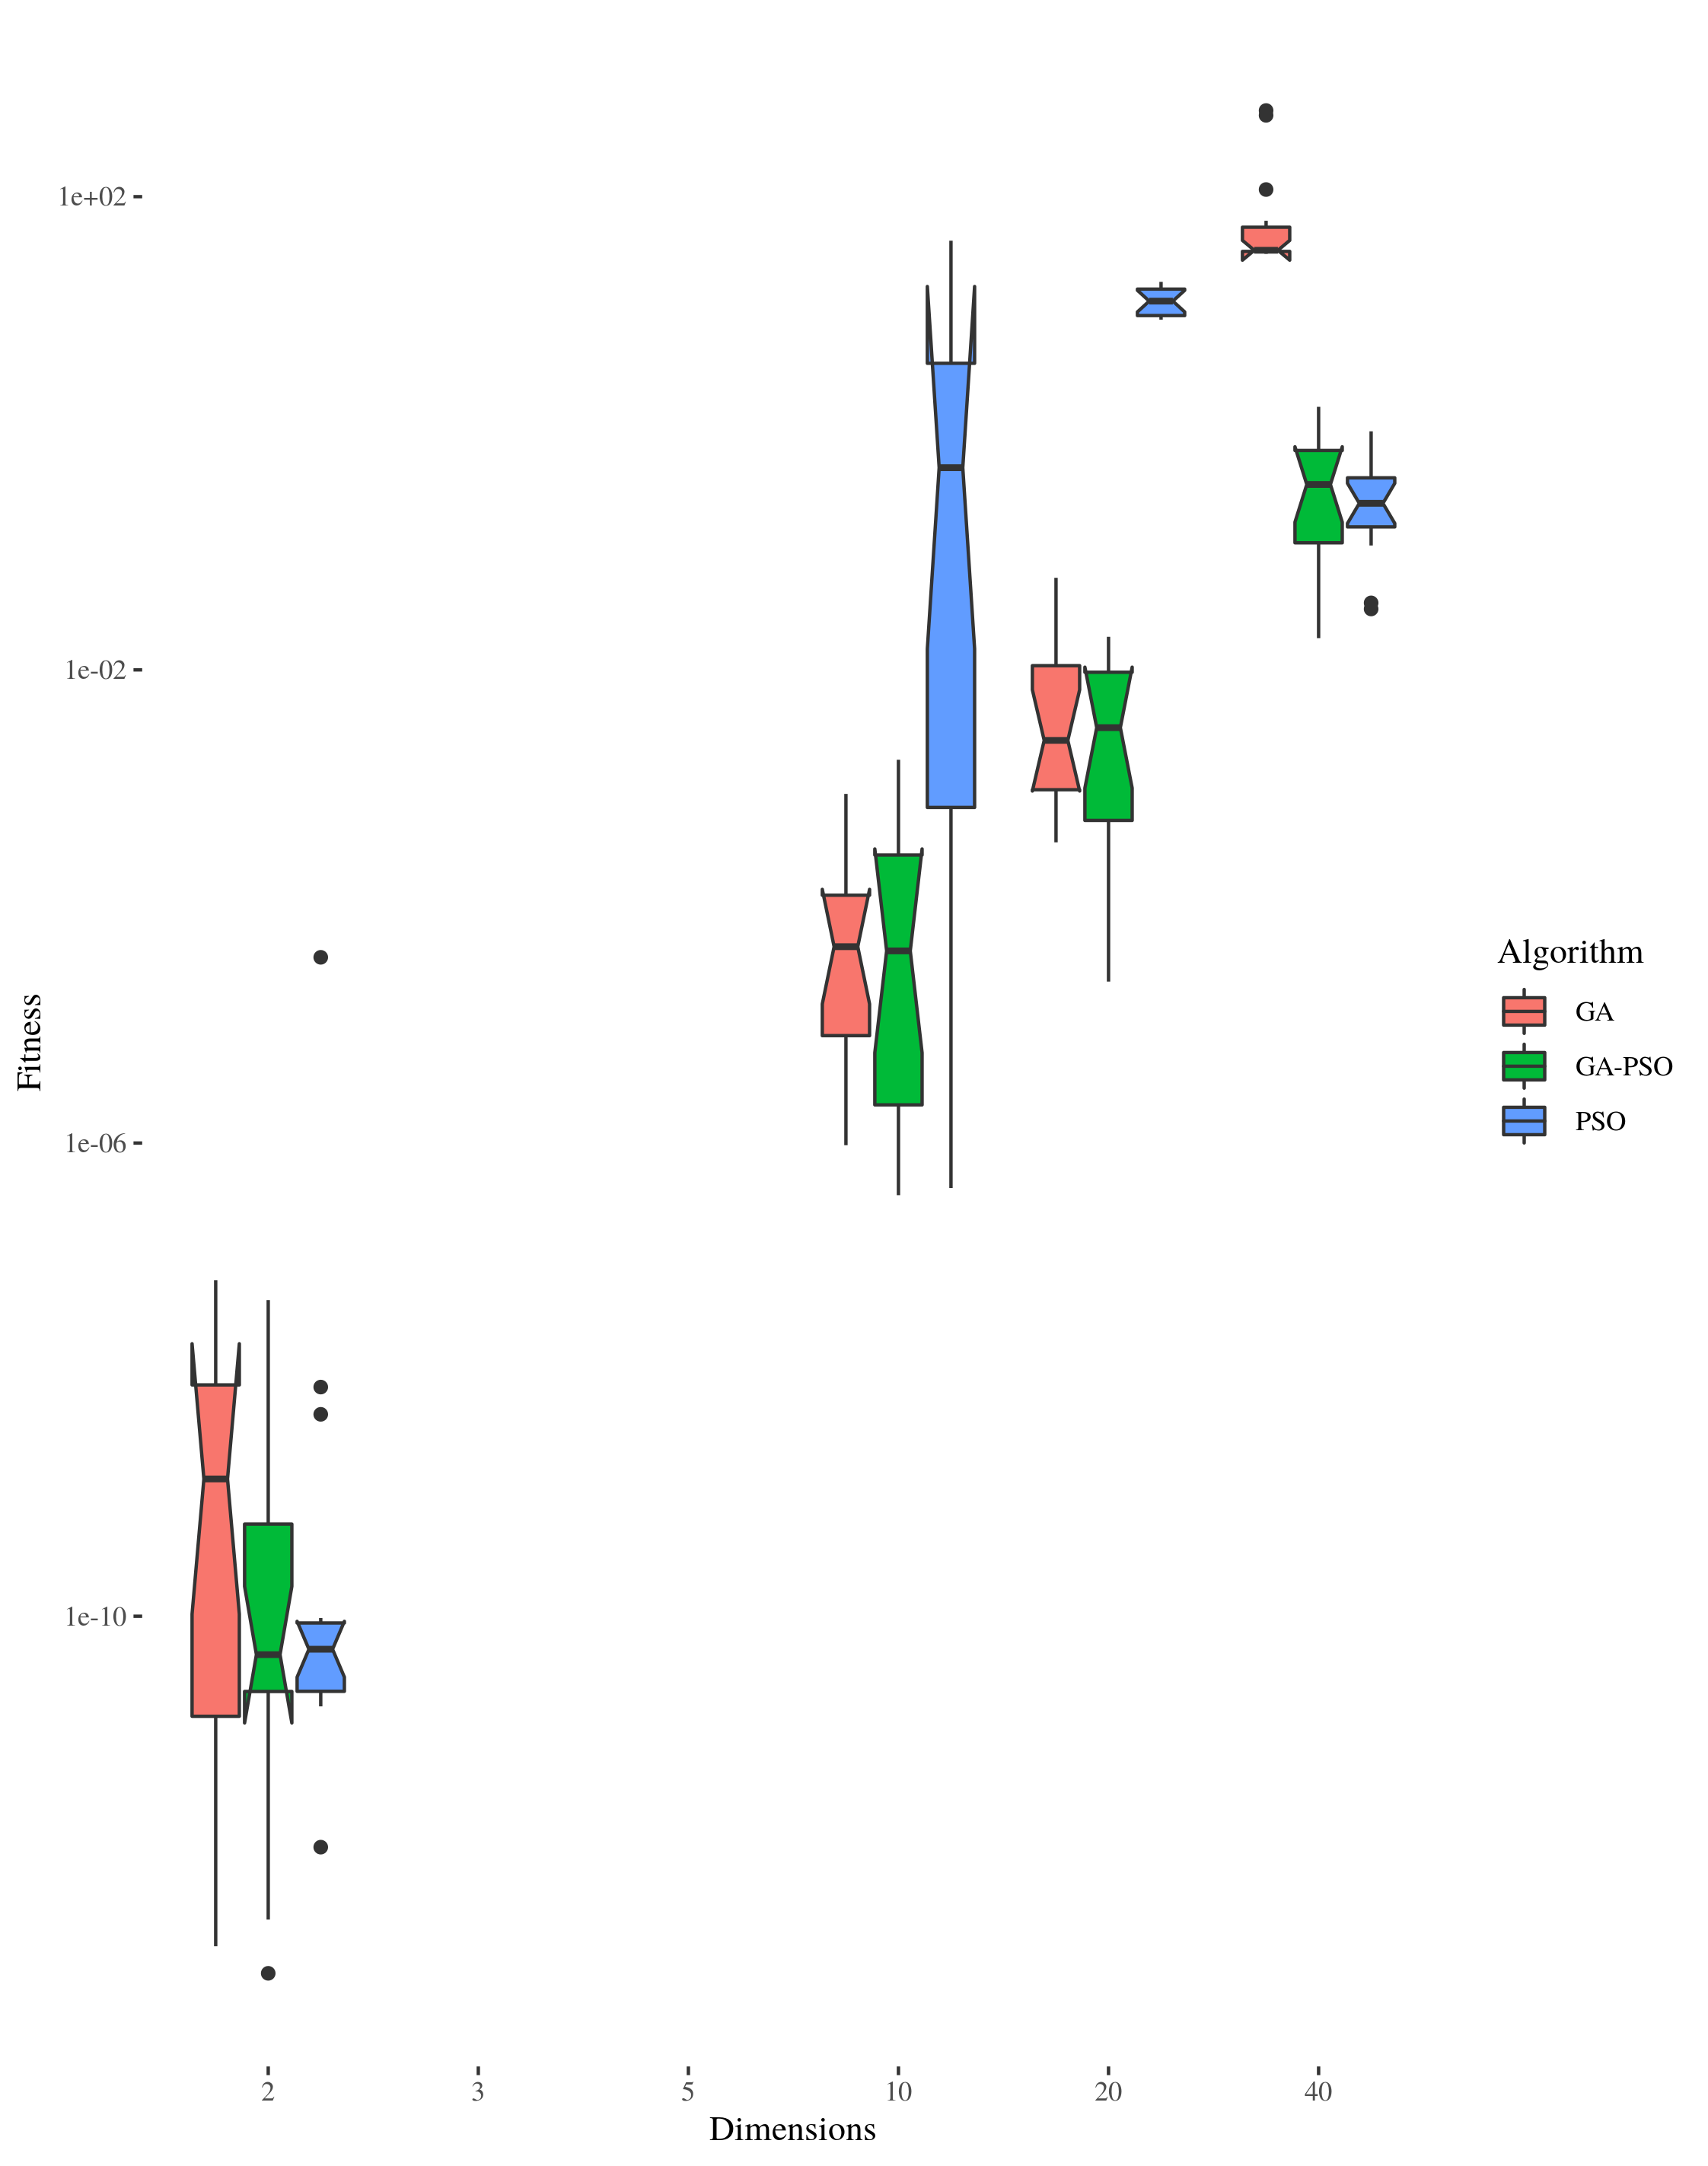
\includegraphics[height=0.4\textheight]{img/rosenbrock-boxplot.png}
  \caption{Boxplot of results for the Rosenbrock function; $y$ axis is logarithmic.\label{fig:boxplot:rosenbrock}}
\end{figure}
%

Finally, averages for GA-PSO show little difference with the best
average in the Rosenbrock function, as shown in Figure
\ref{fig:boxplot:rosenbrock}. In the cases its average is not the
lowest; the difference with the highest average is not significant.

These three functions show a different behavior; however, in most
cases GA-PSO outperform the single-breed algorithms, and in some cases
it shows an average behavior that is not significantly different from
the best. We will discuss this findings in the next section.

\section{Conclusions and future work}

In this paper we have proved how a cross-breed algorithm algorithm,
which uses GA and PSO; can be easily implemented using it. The
cross-breeding actually occurs, allowing these combined algorithms
outperform, with a high probability, single-algorithm
versions. The framework we have provided also has few parameters to
tune, since single-algorithm parameters are selected randomly; in
general, this will boost diversity of every algorithm by itself. 

Since we are using a serverless architecture, high-performance is
achieved, each single experiment lasted between 30 to 40 seconds.
And the whole set of experiments took about 3 hours to complete.
% comment something on the overall time needed for each
% experiment. - JJ
Scalability has as only ceiling the amount of individuals memory can
hold, but its main advantage is that the architecture itself is able
to accommodate as many sub-populations as we need. The limits is
something that we will need to explore in the future. 

The results obtained are probably due to the increased diversity
cross-breed algorithm bring, boosting exploration without sacrificing
exploitation; since results obtained by 
the two intervening algorithm are slightly different, the intermediate
disturbance hypothesis, which has been used to explain results in PSO
\cite{gao2013particle} as well as evolutionary algorithms
\cite{merelo2008testing},  helps keep diversity high. However, in
cases 
where the results for GA and PSO are quite dissimilar, as is the case
for the Sphere function, the cross-breed algorithm might, in some very
specific cases, obtain worse results than the cross-breed  GA-PSO
algorithm. However, the maintenance of diversity makes this difference
relatively small, and the fact that it works better on the rest of the
cases more than compensates.

To get a continuous improvement it is believed that it is required a sort of
mutation applied to the sub-populations. This mutation would be a swapping type,
taking the algorithm parameters from the best and the worst sub-populations,
increasing the possibilities to get an optimal result, preventing get stuck into
a local optimum. Of course, it is expected to use this architecture using more
algorithms than GA and PSO.

Other futures avenues of research to explore would be to use other
kind of algorithms, such as Estimation of Distribution Algorithms or
Differential Evolution, brought into the mix. Scalability will also be
something we will working on in the future, trying to find what are
its limits and how they depend on the type of problem that is solved.

We also think about implementing an interactive user interface to display the
behavior of the populations and allowing a more accessible and precise analysis
of the algorithm. This interface could be helpful as an educational tool.


\section*{Acknowledgements}

Acks\\
taking this much\\
space

\bibliographystyle{splncs04}
\bibliography{multipopulation}
  
\end{document}
